\chapter*{Blog}
        \addcontentsline{toc}{chapter}{Blog}
        \chaptermark{Blog}
	\markboth{Blog}{Blog}
	
	This is the portion of the thesis that I will update regularly with rough notes, lit reviews, results, etc. some of which will be worked in to the real document after some polishing. 
	\section{Goals}
	\begin{itemize}
	\item{10/14: Define specific problem.}
	\item{By Winter Break: Lit Review Complete}
    \item{Before Spring Break: Take Data}
	\end{itemize}

	
	
	\section{To Do}
	\begin{itemize}
	\item{Figure out citations. 12/23/14}
     \item{Take Sample Data Run. Migul 12/2/14}
     \item{Learn de Broglie's interpretation of QM. Miguel 11/6/14}
	\end{itemize}
	
	\subsection{Done}
	\begin{itemize}
	 \item{Set up Accelerometer (Finally--ugh). Miguel 
 2/20/15}
     \item{Get New Silicone Oil. Miguel 1/10/15}
     \item{Send copy of Lit Rev to Daniel to proofread. 12/23/14}
	\item{Find walking regime. Miguel 11/20/14}
	\item{Order Accelerometer. Miguel 11/6/14}
	\item{Learn Basics of Bohmian Mechanics. Miguel 10/28/14}
	\item{Make tray. Miguel 10/20/14}
	\item{Sort out camera situation. Miguel 10/20/14}
	\item{Obtain flashdrives.    Miguel 9/30/14}
	\item{Learn how to use the new \LaTeX\ and Github setup. Miguel 9/30/14}
	\end{itemize}
	
	\section{Literature Review}
	
(Important: Particle-wave association on a fluid interface (Protiere 2006)).
	    
	    In 2005, Yves Couder showed that bouncing oil drops on vertically vibrating fluid bath exhibited properties analogous to the paradoxical properties seen only at the quantum scale (CITE: Dynamical phenomena:  Walking and orbiting droplets?). Couder, John Bush, and others have shown that this system can reproduce double-slit single-particle interference, orbiting, tunneling, quantized orbits, spin, and more. The trajectory of the droplet can be modeled mathematically, and the dynamics of the walker have similarities to de Broglie's theory of quantum mechanics (CITE: Bush 2015).
	    
	    The literature review will begin with a description of Faraday waves and the basic dynamics of a bouncing droplet and a walking droplet. Then we will describe in detail a few of the important quantum-like properites of this system. 
	    
	    	    \subsection{Faraday Waves}
	    
	    
	?

	    
	    \subsection{Bouncing Droplets}
	    Though it had been around for at least a century, the phenomena of droplets bouncing on a vibrating fluid bath was first explained by Jearl Walker in 1978 CITE: WALKER. The first experiments looked at water droplets (bouncing on a vibrating water bath) that persisted for several seconds. Adding detergent to the water and modifying the frequency of vibration increased droplet's lifetime to minutes. Conversely any particulate impurities descrease the droplet's lifetime. Walker concluded that the droplets failed to coalesce because a layer of air trapped between the droplet and the bath would keep the two separate.\footnote{Reedie ??? wrote his thesis titled: ``???" on this very topic! } In other words, the droplet bounces on a cushion of air.
	        
	    %(NONCOALESCENCE AND NONWETTING BEHAVIOR OF LIQUIDS
%Annual Review of Fluid Mechanics
%Vol. 34: 267-289 (Volume publication date January 2002)
%DOI: 10.1146/annurev.fluid.34.082701.154240
%G. Paul Neitzel1 and Pasquale Dell'Aversana2
%)

	    
	 
	    
	    	    \subsection{Walking Droplets}
	    
	       It was Couder who then showed that an oil droplet could live for much longer. Long lifetimes meant that the focus could shift from how the doplet bounced (short time scale) to its interactions with other droplets and its motion (longer time scale).
	       
	       Every time the droplet impacts the bath, it creates a radial traveling wave. If the bouncing droplet impacts the wavefield in such a way that it recives a lateral force from the slope of the wave, then it will be pushed to the side slightly. The next time the droplet makes contanct with the bath, it will again make contact with a slope, and be pushed to the side. This propels the bouncing droplet, causing it to ``walk" across the surface of the bath. These ``walkers" turned out to have particularly interesting behaviours. Indeed, in 2006 Yves Couder and Emmanuel Fort showed that these droplets mimicked the behavior of electrons in the hallmark experiment of quantum weirdness: the double slit experiment. This was the first time that microscopic scale behavior had ever been seen at a macroscopic level, and it sparked interest in the experiment.
	    
	    
	    \subsection{Macroscopic Quantum Scale Behaviors} 
	    \subsubsection{Basic Parameters}
	       Consider a fluid of density $\rho$, viscosity $\nu$, and surface tension $\sigma$, in a bath of depth $H$ driven vertically at an amplitude $A_0$ at frequency $f=\omega/{2\pi}$. By defining $\mathnormal{\gamma}=A_0\omega^2$, the effective gravity in the frame of reference of the bath is $g+\gamma~\mathrm{sin}(\omega t)$. 
	       
	   \begin{figure}[h]
	       \centering
	    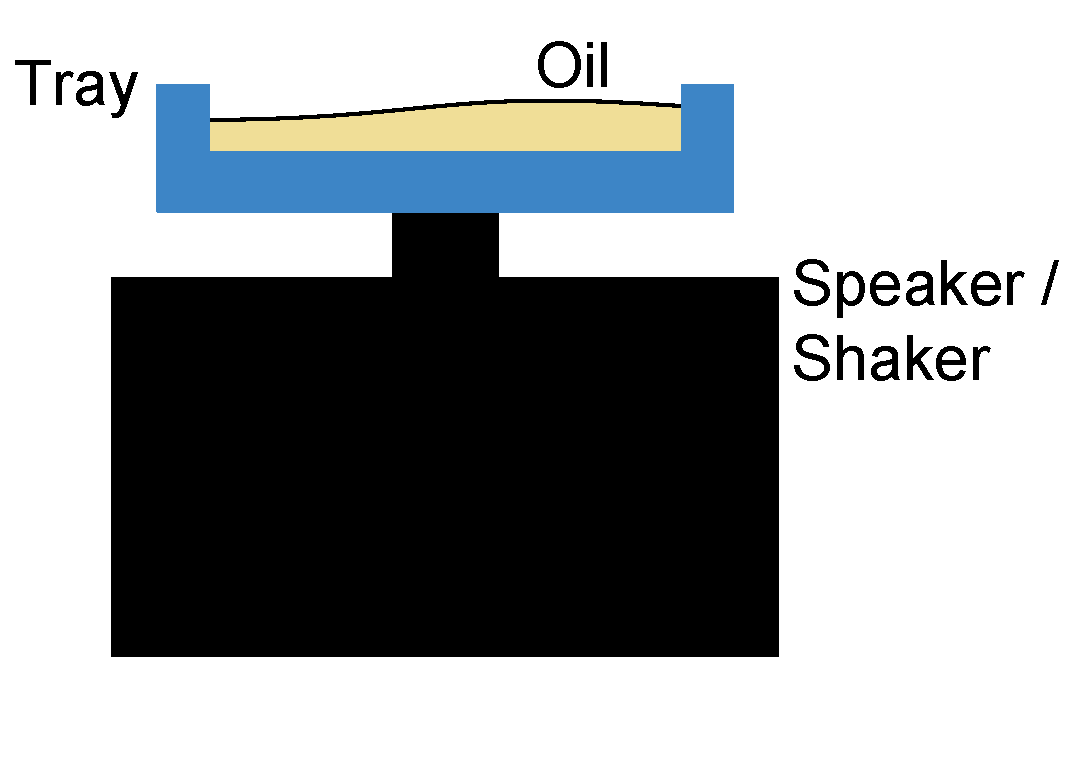
\includegraphics[scale=0.35]{HQASetup.pdf}
	     \caption{The experimental setup. The tray vibrates with an amplitude $A_0$.}
	 \label{regime}
	\end{figure}
	       
	       The oil droplet of diameter $D$ bounces in the regime $\gamma<\gamma_F$, where $\gamma_F$ is the Faraday threshold (at this point, Fraday waves appear). The important experimental limits are outlined in \refTab{approxlimits}. 
	       \begin{table}[htdp] 
\caption[Basic Table 1]{Approximate Limits for Bouncing Drop Behavior} 
\begin{center} 
\begin{tabular}{c c c} 
\toprule 
  Parameter &  Lower Limit & Upper Limit \\
  \midrule
Viscocity $\nu$ (cSt) & 10 & 100 \\ 
Bath Depth $H$ (mm) & 4 & 10 \\
Frequency $f$ (Hz) & 20 & 150 \\
Amplitude $A_0$ (mm) & 0.1 & 1 \\
Drop Diameter $D$ (mm) & 0.6 & 1.0 \\
\bottomrule 
\end{tabular}
\end{center}
\label{approxlimits} 
\end{table}	

For certain parameters, the bouncing drop will behave differently. The vibration number describes ``the relative magnitude of the forcing frequency and the drop's natural oscillation frequency," and is given by:
	       	      
\begin{equation} \label{vibrationnumber}
V_i = \frac{\omega}{2}\sqrt{\frac{\rho D^3}{2\sigma}}
\end{equation}   	       	       
	       	       The natural frequency of the droplet occurs around $V_i = 0.65$, where the droplet can exhibit both walking and bouncing behaviors. Setting up a plot with $V_i$ on the y axis and (dimensionless) ${\gamma}/{g}$ on the x axis can help in showing the behavior of the droplet, shown in \refFig{regime}. 
	    
	    \begin{figure}[h]
	% the options are h = here, t = top, b = bottom, p = page of figures.
	% you can add an exclamation mark to make it try harder, and multiple
	% options if you have an order of preference, e.g.
	% \begin{figure}[h!tbp]
	   
	       \centering
	    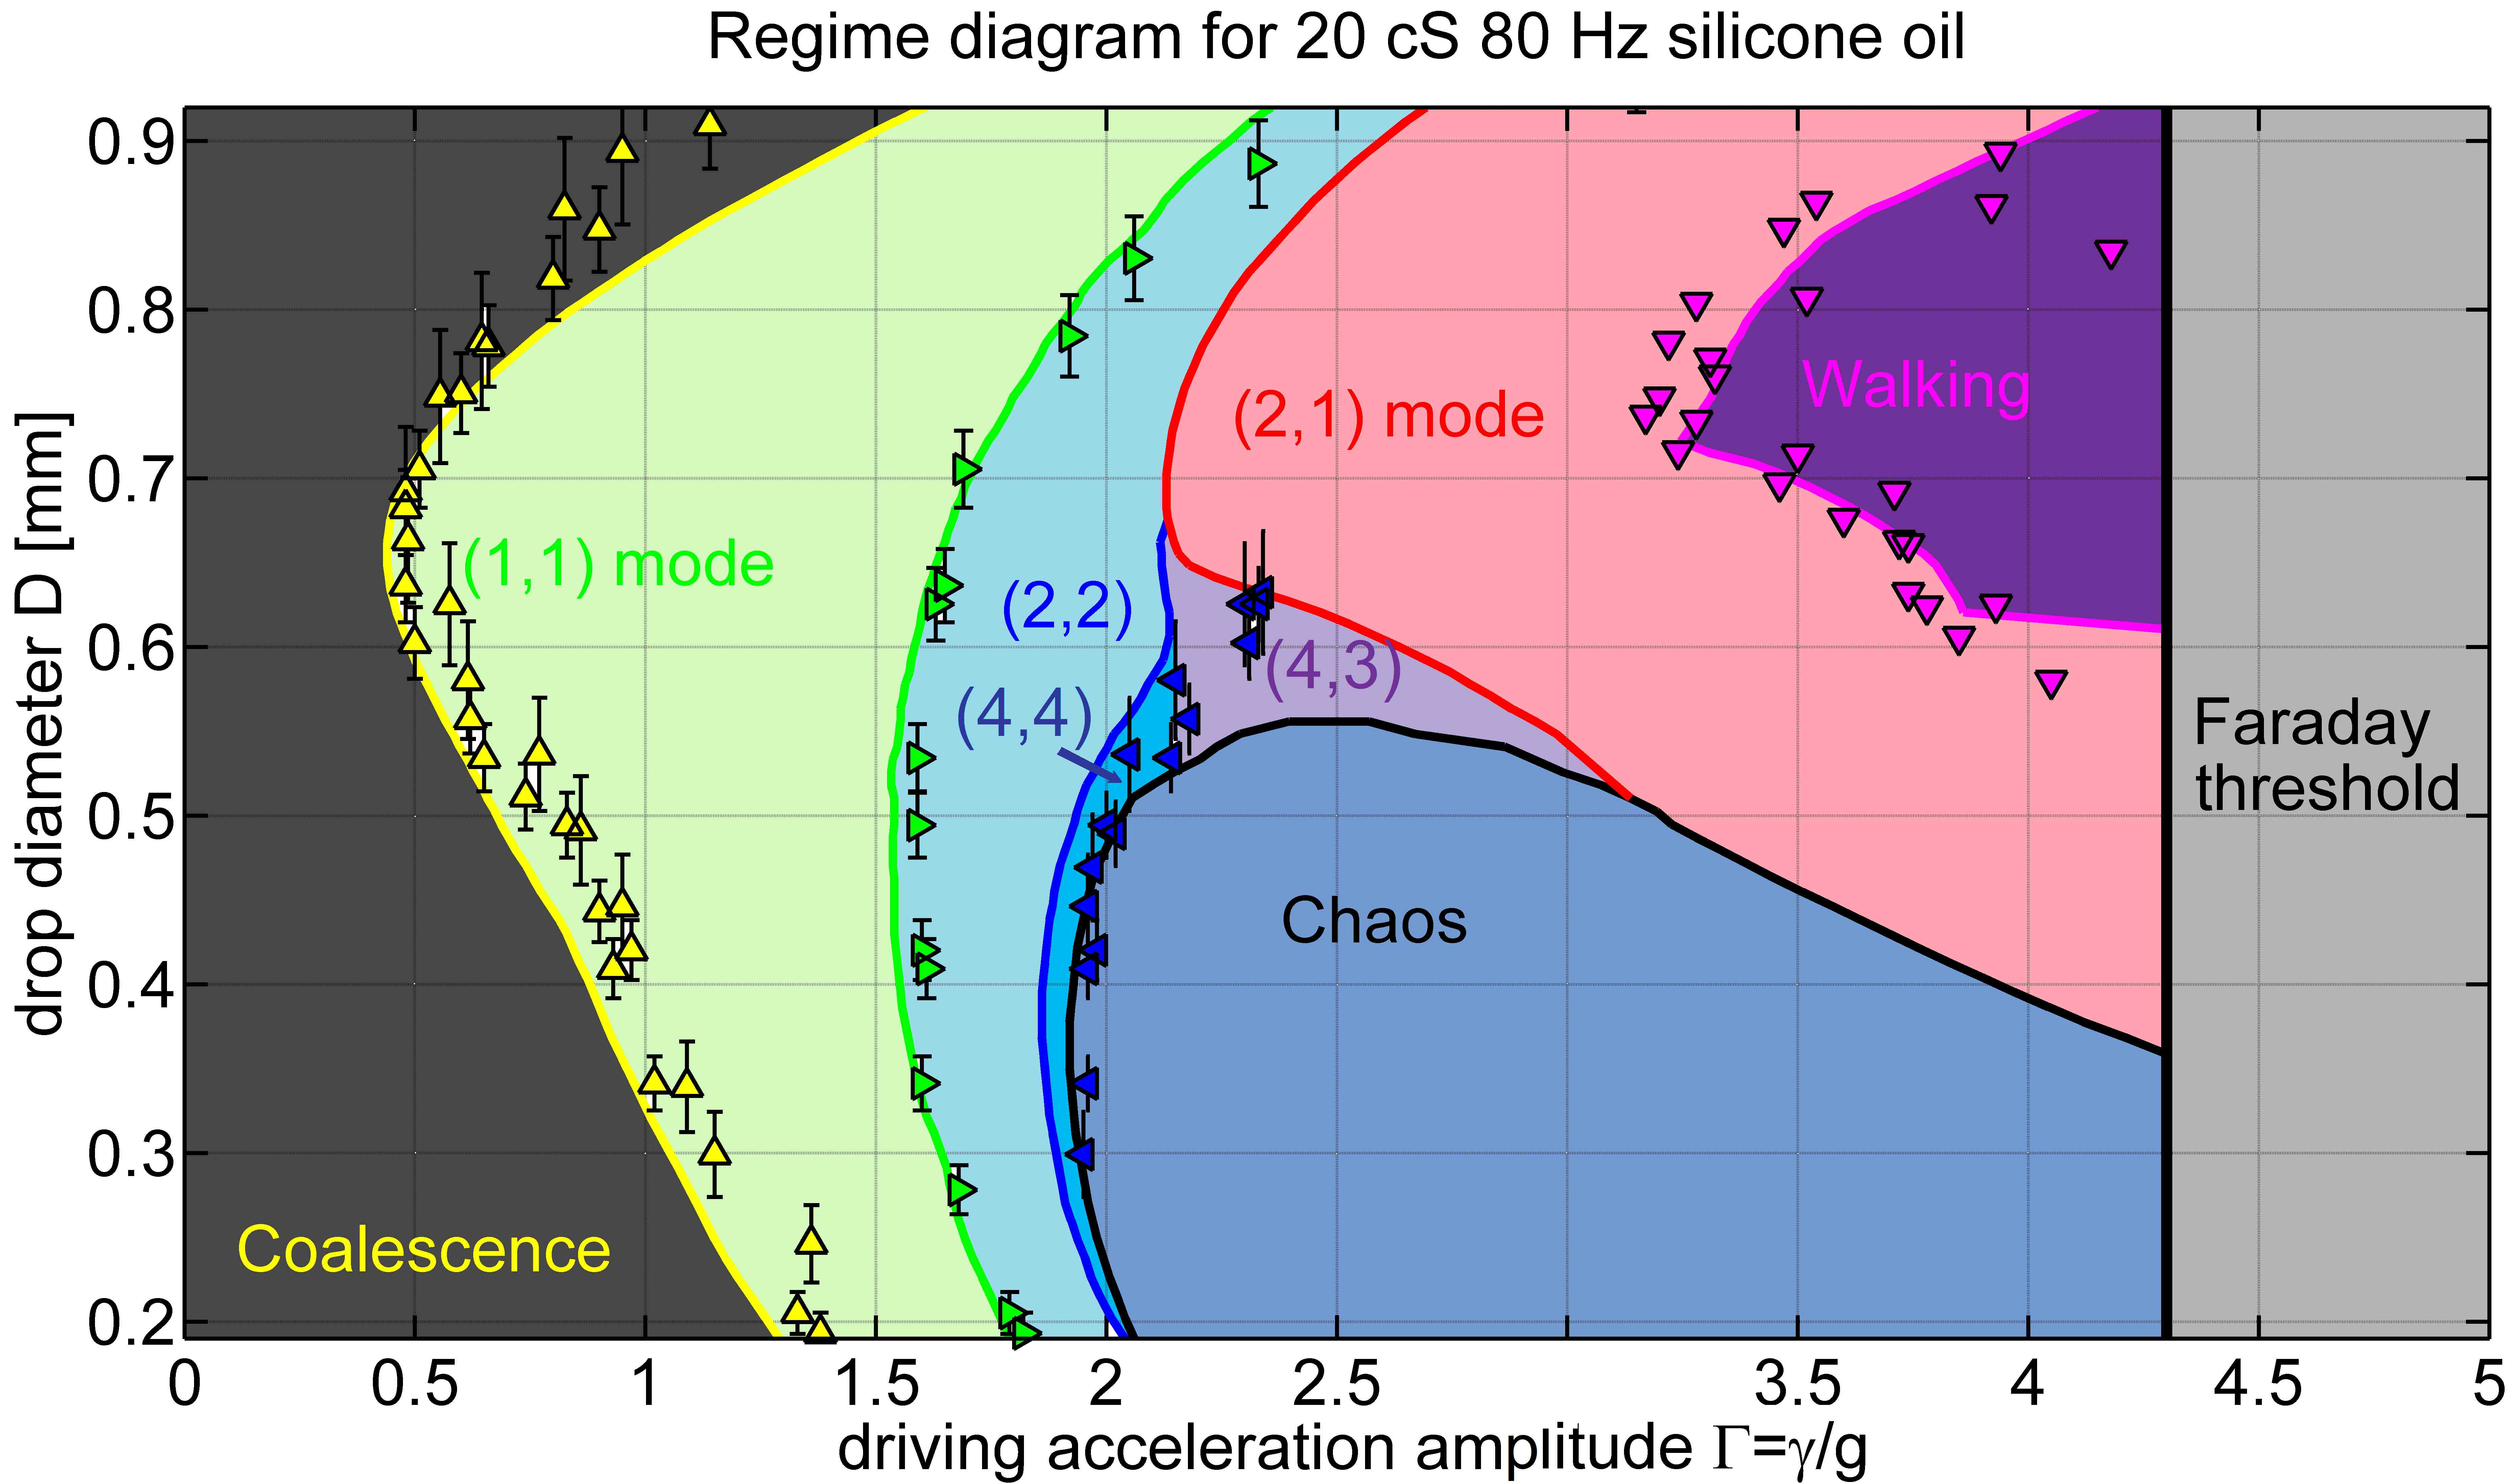
\includegraphics[scale=0.075]{Regime-Mega}
	     \caption{The different bouncing regimes for the oil drops of 20 cS silicon oil and at $f$ = $\omega / 2\pi$ = 80 Hz. The parameters ($m$,$n$) describe the droplet that bounces $n$ times in $m$ forcing periods. }
	 \label{regime}
	\end{figure}

The various modes seen in \refFig{regime} can be described by ($m$,$n$), where $n$ is the number to times the droplet contacts the surface over period $m/f$. For example, in the (1,1) mode, the droplet hits the oil bath once per driving period. In the (2,2) mode, the drop makes two bounces of differing heights. 
	       
            \subsection{Path Memory}
                        
            Path memory is a parameter that can be varied in this setup; it is essentially the damping of the system. Every time the droplet impacts the bath, it creates a radial traveling wave. Over the course of many bounces, a wavefield composed of a superposition of the many waves arises. In this way the wavefield ``remembers" previous interactions. Because droplet motion is influenced by the wavefield, controlling the damping of the wavefield will influence the path of the walker. The heavily damped system has a low memory, while undamped system correspends to higher memory. As one gets closer to the Faraday threshold, one achieves higher and higher memory because waves last for longer. The quantum like features of this experiment arise in the high-memory limit. (For more, Eddi et. al, 2011b: Information stored in Faraday waves.) 

            \subsection{Bound States}
            A bouncing droplet creates a damped wave that depends on the driving acceleration (${\gamma_m}/ g$) CITE: Protiere 2005. A periodic damped wave allows for two bouncers to form a ``bound state".  Starting far away from one another, the two droplets drift towards one another until a fixed distance $d_{0}^{bd}$. Increasing driving acceleration will decrease the value of $d_{0}^{bd}$. These bound bouncers form triangular lattices, and their periodicity is highly sensitive to the mass of the droplet. (LOOK AT EDDI ET ALL 2008).
            
            Walkers can also form bound states. Two walkers of the same size that are approaching one another can form an orbit around their center of mass. Between the two droplets is the fixed distance $d_{n}^{orb}$ given by
            
\begin{equation} \label{orbital}
d_{n}^{orb} = (n - \epsilon_0)\lambda_F
\end{equation}         
where $\epsilon_0$ is a fixed distance which is the same for all orbitals of these walkers (usually in the range $0.15 < \epsilon_0 < 0.25$ depending on droplet diameter), and $n = 1,2,3$... for drops that are in phase or $n = 1/2, 3/2, 5/2$... for drops out of phase. Orbiting periods are approximately porpotional to $d_{n}^{orb}$, which ends up meaning that the velocity of the orbiting walkers is a little less than the velocity of a free walker CITE: Protiere 2006. Orbiting of different sized droplets can also arise.      

            \subsection{Scattering States}
            Two identical walkers headed towards each other can form fixed orbits, or they can scatter. The droplets are deflected through their wavefields (they never actually make contact with one another)            
            \subsection{Single-Particle Diffraction}
In 2006 Couder and Fort showed that the system had properties that were strikinly similar to two famous and controversial quantum experiments (Couder and Fort, 2006). They were able to demonstrate that a single walker travelling through one slit seemed to have its direction altered seemingly randomly, before continuing forward on its new path. By statistically analyzing many trials, Couder and Fort showed that the histogram of the ``diffraction" actually resulted in a diffraction pattern strikingly similar to the single photon diffraction experiment performed by Taylor in 1909. 

Next, Couder and Fort added a second slit next to the first one. Now a single walker could pass through  one of two slits, and it was discovered that a histomgram of this data returned another diffraction pattern. This result is of course reminiscent of one of the most famous experiments in physics: Young's double slit diffraction with photons and electrons. 
    
Using a numerical simulation, Couder and Fort were able to reproduce similar results. 
    
As Couder and Fort mention in their paper: ``A discussion of the relation between these single-particle experiments and those concerning elementary particles is unavoidable." Important differences and similarities are then described between the quantum system and the quantum-like system. For the differences: we have a dissapative system, where energy is continually put in through the vibration of the tray; the particle can be followed;\footnote{C and F note that it'd be impossible to dectect the particle without disturbing it "by any means at its scale," like a bouy, for example. As the bouy floated it would interfere with the system by altering the wave pattern on the surface.} it's really effectively moving in two dimensions; the velocity is measurable; and the probability distributuion is linked with the wave amplitude (rather than it's intensity). And then of course, the similarities: an uncertainty priciple arises from the statistical data (and without knowledge of the actual paths followed by the walkers); and some others that were unclear...

Recently, Harris attempted to reproduce single slit interference. With better technology, new results were found. Using a looping guiding batt, trajectories were found to follow the same loop without deviating. Only at a very high memory were there chaotic paths.
	       \subsection{Tunneling}
	       The guiding wave field can be partially reflected off of an edge or even a change in depth of the oil bath. This effect can be seen when a walker is pushed back from a under-the-surface step, seemingly without any contact. In rare cases, the walker will actually tunnel across the step; that is, it will continue to walk along the surface of the oil bath and pass over the step without reflection. In the first experiment done by Eddi et al., they demonstrated tunneling by by building square ``corrals" of varying thicknesses. In the second experiment, they built a rhombus shape which forced the walker across the center of a rhombus. The barrier was placed perpendicular to the direction of travel of the walker, so that it would hit the wall directly rather than at an angle (as in the square corral). ``The tunneling probability decreases exponentially with the barrier width and increases as the Faraday threshold is approached." Eddi et. al also found that the probability of tunneling increased with the velocity of the walker. (For more, Eddi et. al 2009b: Unpredictable Tunneling of a classical wave-particle association.)
	       
	       
	        The unpredictability of the tunneling comes from the complex interatction between the drop and its guiding wave. 

\subsection{Motion in a Confined Geormetry}
By tracking the droplet as it bounces around the tray over a period of time, one can look at the overall statistical behavior of the droplet. Two experiments tracked walkers in an experimental coral (Harris and Bush, 2013, Harris et al. 2013) in the high-memory, chaotic motion regime. A histogram of the statistical data shows that the "probability of finding a walker at a given point in the corral is roughly prescribed by the amplitude of the Faraday wave mode of the cavity at the prescribed forcing frequency."

Quantum corral experiments performed by Crommie et al. (Crommie et al. 1993 a b) present similar findings. In the experiment, electrons were confined in a Cu(III) substrate using barriers of iron adatoms. Using tunneling spectroscopy, the electrons were found to have a specific resonances depending on the corral shape. As in the case of Harris' circular corral experiment where the corral and the Faraday wavelength, $\lambda_F$, dictate the wavelike statistical patter, in the quantum experiment the corral and the \textit{de Broglie} wavelength, $\lambda_{dB}$, dictate the form of the wavelike statistical pattern. 

\subsection{Walker Trajectories}
In the regime of walkers we have $R_e \sim 20$, $B_0 \sim 0.1$, and $W_e \sim 0.1$. For the millimeric walkers, the dominant force comes from impact of the curvature of the surface. Gilet and Bush (2009: Chaotic bouncing of a drop on a soap film, and the fluid trampline: droplets bouncing on a soap film) show that the surface of the vibrating oil can be modeled with a soap film, where the soap film acts like a linear spring. 

As the oil bath is forced up and down, a tiny droplet of oil will ``walk" across the surface. Mol\'{a}\v{c}ek and Bush have developed an equation of a droplet that describes the trajectory of the walking droplet, ignoring the verical dynamics by time averaging them out (cite: J. Mol\'{a}\v{c}ek and J. W. M. Bush, ``Drops walking on a vibrating bath: towards a hydrodynamic pilot-wave theory" J. FluidMech. 727, 612-647 (2013).). The trajectory of the walking droplet of mass $m$ at position $\textbf{x}(t) = (x(t),y(t))$ is given by
\begin{equation}
m \ddot{\textbf{x}} + D \dot{\textbf{x}} = -mg\nabla h(\textbf{x},t) 
\end{equation}
where $D$ describes the drag coefficient and $h(\textbf{x},t)$ describes the shape of the wavefield. Thus the second term describes the time averaged drag from both the flight and the impact of the droplet (as usual, depends on the velocity), and the third term describes the propulsive wave force resulting from drops landing on the inclined wave surface. 

The wavefield is quite complicated because it depends on the memory. For a single impact of a droplet, Oza et al. argue the surface wave can be approximated with an integral of a monochromatic radial Bessel function of the first kind

\begin{equation}
h(\textbf{x},t) = \frac{F}{T_F} \int_{-\infty}^{t} J_0 \frac{(k_F |\textbf{x}(t)-\textbf{x}(s)|)}{|\textbf{x}(t)-\textbf{x}(s)|} (\textbf{x}(t)-\textbf{x}(s))e^{-(t-s)/(T_F M_e)} ds
\end{equation}
with $F$ giving the wave force coefficient (estimated in the above source), $T_F$ describing the Faraday period, and $k_F$ describing the Faraday wave number determined by the Faraday wavelength $\lambda_F = 2π/k_F$ (integral from A. U. Oza, D. M. Harris, R. R. Rosales, and J. W. M. Bush, "Pilot-wave dynamics in a rotating frame: on the emergence of orbital quantization" J. Fluid Mech. 744, 404-429 (2014).). (Faraday was a popular guy.) Finally, that last term $M_e$ is the nondimensional memory parameter $M_e = T_d/[T_F(1-\gamma / \gamma_F)]$ (with $T_d$ being the unforced decay time).

\section{Experimental Setup}

\section{Bohmian Mechanics}

\subsection{Formalism}
\subsubsection{The Schroedinger Equation and $\psi$}

We begin with the Schoedinger equation

\begin{equation}
i \hbar \frac{\partial}{\partial t}\psi = \hat H \psi
\end{equation}
where $\hat H$ is the Hamiltonian and $\psi$ is the wavefunction. The Hamiltonian can be expanded (assuming there is no electric field) to give

\begin{equation}
\label{SE}
i\hbar\frac{\partial}{\partial t} \psi(\mathbf{x},t) = \left [ \frac{-\hbar^2}{2 m}\nabla^2 + V(\mathbf{x},t)\right ] \psi(\mathbf{x},t)
\end{equation}
where $V(\mathbf{x},t)$ is the potential energy of the system. The solution $\psi$ is of the form:

\begin{equation}
\psi(\mathbf{x},t) = R(\mathbf{x},t) e^{i S(\mathbf{x},t) / \hbar}
\end{equation}
where $S$ and $R$ are real. Plugging in our equation for $\psi$ into the Schoedinger equation (\refeq{SE}) will produce two separate equations: one giving the time derivative of $R$ and the second giving the time derivative of $S$. From these equations, a Hamilton-Jacobi equation can be written for a quantum system.
    Let's begin by computing the left hand side of \refeq{SE} in terms of $R$ and $S$.   

$$
\begin{align*}
i\hbar\frac{\partial}{\partial t} \psi(\mathbf{x},t) &= i \hbar\left(\frac{\partial R}{\partial t} e^{i S / \hbar} + R \frac{i}{\hbar}\frac{\partial S}{\partial t} e^{i S / \hbar}\right)
\\ &= i \hbar \left(\frac{1}{R} \frac{\partial R}{\partial t} + \frac{i}{\hbar}\frac{\partial S}{\partial t}\right) \psi(\mathbf{x},t) 
\\ &= \left(i \hbar \frac{1}{R} \frac{\partial R}{\partial t} - \frac{\partial S}{\partial t}\right) \psi(\mathbf{x},t)
\end{align*}
$$
Let's leave that alone for a little bit, while we focus on the right hand side of \refeq{SE}. Since it's a little more complicated, we will start with one term of the right hand side:

$$
\begin{align*}
\nabla^2 \psi(\mathbf{x},t)  &= e^{i S / \hbar} \nabla^2 R + \left(\frac{i}{\hbar}\right)^2 (\nabla S)^2 R e^{i S / \hbar} + \left(\frac{i}{\hbar}\right) R e^{i S / \hbar} (\nabla^2 S) + \left(\frac{2i}{\hbar}\right) (\nabla R \cdot \nabla S) R e^{i S / \hbar}
\\ &= \left(\frac{\nabla^2 R}{R} - \left(\frac{\nabla S}{\hbar}\right)^2  + \left(\frac{i \nabla^2 S}{\hbar}\right) + 2 i \left(\frac{\nabla R \cdot \nabla S}{\hbar}\right) \right) \psi(\mathbf{x},t) 
\end{align*}
$$

Now the hard part is done, and we can say that the right hand side of \refeq{SE} is given by 

$$
\begin{align*} 
\left [ \frac{-\hbar^2}{2 m}\nabla^2 + V(\mathbf{x},t)\right ]\psi(\mathbf{x},t) &= \left [-\frac{\hbar^2  \nabla^2 R}{2 m R} + \left(\frac{(\nabla S)^2}{2 m}\right)  - i \hbar \left(\frac{\nabla^2 S}{2 m}\right) - i \hbar \left(\frac{\nabla R \cdot \nabla S}{m}\right) + V(\mathbf{x},t) \right]\psi(\mathbf{x},t) 
\end{align*}
$$

Ok, now that we've got that done, the next part will be super easy. Starting with Schrodinger's equation and plugging in left and right hand sides we calulated seperately. 

$$
i\hbar\frac{\partial}{\partial t} \psi(\mathbf{x},t) = \left [ \frac{-\hbar^2}{2 m}\nabla^2 + V(\mathbf{x},t)\right ] \psi(\mathbf{x},t)
$$
$$
\left(i \hbar \frac{1}{R} \frac{\partial R}{\partial t} - \frac{\partial S}{\partial t}\right) \psi(\mathbf{x},t) =\left [-\frac{\hbar^2  \nabla^2 R}{2 m R} + \left(\frac{(\nabla S)^2}{2 m}\right)  - i \hbar \left(\frac{\nabla^2 S}{2 m}\right) - i \hbar \left(\frac{\nabla R \cdot \nabla S}{m}\right) + V(\mathbf{x},t) \right]\psi(\mathbf{x},t) 
$$
Now we can divide out $\psi$ from both sides
$$ 
i \hbar \frac{1}{R} \frac{\partial R}{\partial t} - \frac{\partial S}{\partial t} = -\frac{\hbar^2  \nabla^2 R}{2 m R} + \left(\frac{(\nabla S)^2}{2 m}\right)  - i \hbar \left(\frac{\nabla^2 S}{2 m}\right) - i \hbar \left(\frac{\nabla R \cdot \nabla S}{m}\right) + V(\mathbf{x},t)
$$
and group the imaginary numbers on the left side and the real numbers on the right side 
$$ i \hbar \frac{1}{R} \frac{\partial R}{\partial t} + i \hbar \left(\frac{\nabla^2 S}{2 m}\right) + i \hbar \left(\frac{\nabla R \cdot \nabla S}{m}\right) = \frac{\partial S}{\partial t} -\frac{\hbar^2  \nabla^2 R}{2 m R} + \left(\frac{(\nabla S)^2}{2 m}\right)  + V(\mathbf{x},t)
$$
Recall that both $S$ and $R$ are real. Note that the only way for all of the imaginary terms to equal all of the real terms is if they both equaled zero.
$$i \hbar \left(\frac{1}{R} \frac{\partial R}{\partial t} + \frac{\nabla^2 S}{2 m} + \frac{\nabla R \cdot \nabla S}{m}\right) = \left(\frac{\partial S}{\partial t} -\frac{\hbar^2}{2m}\frac{\nabla^2 R}{R} + \frac{(\nabla S)^2}{2 m}  + V(\mathbf{x},t) \right) = 0
$$
This then gives us two sepeate equations, one for the time derivative of $R$ and another for the time derivative of $S$.

\begin{equation}
\label{dR/dt}
\frac{\partial R}{\partial t} = -\frac{R}{2 m}\left(\frac{\nabla^2 S}{m}-2\nabla R \cdot \nabla S\right)
\end{equation}


\begin{equation}
\label{dS/dt}
\frac{\partial S}{\partial t} = \frac{\hbar^2}{2m}\frac{\nabla^2 R}{R} - \frac{(\nabla S)^2}{2 m} - V(\mathbf{x},t)
\end{equation}

What does this do for us? Both equations will provide helpful descriptions of our system.

\subsubsection{The Quantum Potential}

We can rewrite \refeq{dS/dt} in a provokative way 

\begin{equation}
\label{BohmHamiltonian}
- \frac{\partial S}{\partial t} = \frac{(\nabla S)^2}{2 m} + V(\mathbf{x},t) + \frac{\hbar^2}{2m}\frac{\nabla^2 R}{R}
\end{equation}
which should look suspiciously familiar. If I were to tell you that $\nabla S$ had units of momentum and $\partial S/\partial t$ units of energy, then this equation would look a lot like a Hamiltonian! The first term takes care of the kinetic energy, the second is the potential energy term, but we have this mysterious third term which we haven't ever encountered in classical mechanics. If we define this term as our ''quantum potential" 

\begin{equation}
\label{QuantumPotential}
U(\mathbf{x}) =  \frac{\hbar^2}{2m}\frac{\nabla^2 R}{R} = \frac{\hbar^2}{4m}\left[\frac{1}{2} \frac{\nabla^2 P}{P} - \frac{(\nabla P)^2}{P^2}\right] 
\end{equation}
then we really \textit{can} think of \refeq{BohmHamiltonian} as a Hamiltonian with an extra potential term thrown in to make it "quantum." Note that in cases where $\hbar$ is much smaller than the rest of the terms (i.e. not the quantum realm), then this quantum potential term goes away, and we are left with the regular Hamilton equation from classical mechanics. 

Recall that when writing a Hamiltonian, the potential terms govern the forces on the particle. For a conservative system, the force is given by F(x) = -$\partial U/\partial x$. If we include a quantum mechanical potential in our Hamiltonian, then this potential must cause a force on the paticle in addition to the one supplied by the $V(x)$ term. 


\subsubsection{Continuity Equation}
Plugging in the probability density $P(\mathbf{x},t) = R^2(\mathbf{x},t)$ into \refeq{dR/dt} also gives us something quite interesting.

MATH?

which we can finally express as 

\begin{equation}
\label{ProbCurrent}
\frac{\partial P}{\partial t} + \nabla \cdot \left( P \frac{\nabla S}{m} \right)
\end{equation}

In describing the quantum potential term it was mentioned that $\nabla S$ can be thought of as momentum, so then from our classical relationship between momentum and velocity  $\textbf{v}(\textbf{x},t)=\nabla S/m$ can be thought of as velocity. Then by defining the probability current as $j(\mathbf{x},t) = P\nabla S/m$ then we recover

\begin{equation}
\label{ProbCurrent}
\frac{\partial P}{\partial t} + \nabla \cdot j(\mathbf{x},t)
\end{equation}
known as the continuity equation! This tells us that $P$ is conserved over time.

\subsubsection{Finding $R$ and $S$}

